\section{Historische Einführung in die Rastertunnelmikroskopie}
Die ursprüngliche Idee der Erfinder des Rastertunnelmikroskopes
war es nicht, ein Mikroskop zu konstruieren,
sondern Spektroskopie in einer Größenordnung von 
100 \r{A} durchzuführen \cite{binnig1987scanning}.
Mit der ersten experimentellen Realisation \cite{thompson1976thermal}
des Tunnelns mit einer positionierbaren Spitze tauchte das 
das Konzept des Tunnelns in der 
Festkörperphysik auf, als versucht wurde, durch Vakuum bzw. durch
eine Vakuumbarriere zu tunneln \cite{binnig1982tunneling}. 
Erst dann wurde festgestellt, das mit dieser Methode nicht nur
Spektroskopie, sondern eine neue Art des Mikroskops entwickelt werden
konnte.
Diese
waren zunächst aufgrund der Vibrationen nicht erfolgreich. Nun sind
die Vorteile des Vakuumtunnelns aber evident: 
Zum einen handelt es sich um die konzeptuell am einfachsten
herzustellende Barriere, zum anderen ist ein freier Zugang 
der Elektroden für die Untersuchung anderer
physikalischer und chemischer Prozesse möglich.
Die Fragen, die sich in diesem Zusammenhang
ergaben und gelöst bzw. beantwortet werden mussten, waren:

\begin{enumerate}
\item Wie können die mechanischen Vibrationen, die die Spitze
erschüttern und sich gegenseitig aufschaukeln, unterdrückt bzw.
verringert werden?
\item Wie stark sind die (Anziehungs-)kräfte zwischen der Spitze
und der Probe? Wie sollte die Form der Spitze aussehen und wie
ist es möglich eine solche Form auf dieser Skala herzustellen?

\end{enumerate}

1981 führten die Autoren G.Binnig, H.Rohrer,
Ch.Gerber und E.Weibel in Zürich zum ersten Mal ein erfolgreiches
Tunnelexperiment \cite{binnig1982tunneling} 
mit einem justierbarem Vakuum Spalt durch. 
Ziel war hierbei, das Phänomen des Tunnelns so zu erforschen,
um es in der Spektroskopie und andere Methoden einsetzen zu können. 
Offensichtlich war der schwierige Teil der, die Vibrationen,
die vergangene Experimente fehlschlugen ließen, hinreichend zu
unterdrücken, um somit das eigentliche Signal noch identifizieren zu
können. Dies wurde in dem erwähnten Experiment durch eine 
Dämpfung des Tunnelbauteils erreicht, und zwar durch einen Schutz
von akkustischen Rauschen durch eine das Mikroskop umgebende 
Suspension innerhalb einer Vakuumkammer. Mithilfe von Leviation durch
Supraleiter-induzierten Magneten sowie
der Steuerung mit Piezoelementen erreicht. \\ Der Trick liegt darin,
die charakteristischen Frequenzen so zu wählen, dass die 
Eigenfrequenzen des Materials für Vibrationen weit darüber liegen.
Dies ist möglich, indem die Größe des Bauteils sehr klein
skaliert wird, somit können sich keine Vibrationen ausbilden.
Die Frage nach der Form der Spitze ist komplizierter, da es 
nicht unbedingt möglich ist, die Spitze als Sphere mit einer
bestimmten Krümmung und Radius zu beschreiben, da die Rauheit der
Spitze die Existenz vieler kleiner Spitzen implizieren. Diese
sogenannten 'Minispitzen' reagieren sehr sensitiv auf die anliegende
Tunnelstromstärke; die jeweils näheste bildet dann die Verbindung
zur Probe (siehe Abbildung \ref{fig:multitip}).\\ 
\begin{figure}
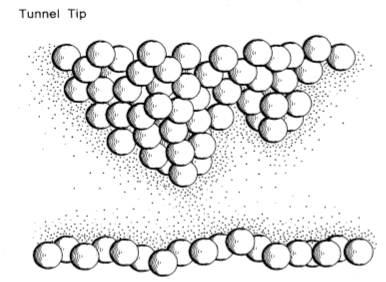
\includegraphics[width=10cm]{pics/multitip}
\caption{ Schematische Abbildung aus \cite{binnig1987scanning}
auf der der die strukturelle Aufbau der Spitzen und der Probe 
zu sehen ist.} 
 \label{fig:multitip}
\end{figure}
Die erste Anwendung, welche die Rastertunnelmikroskopie bekannt
machte, war die Oberflächenrekonstruktion von Silizium(111)  
\cite{binnig1983111} (siehe Abbildung \ref{fig:silicium}).
Dabei handelte es sich um ein offenes Problem in der
Festkörperphysik. Wie sich später durch die experimentelle
Aufarbeitung zeigte, waren die theoretischen Vorhersagen nicht 
korrekt und mussten korrigiert werden, gerade auch deswegen
erlangte die Rastertunnelmikroskopie ab 1985 grosse Bekannheit.
\begin{figure}
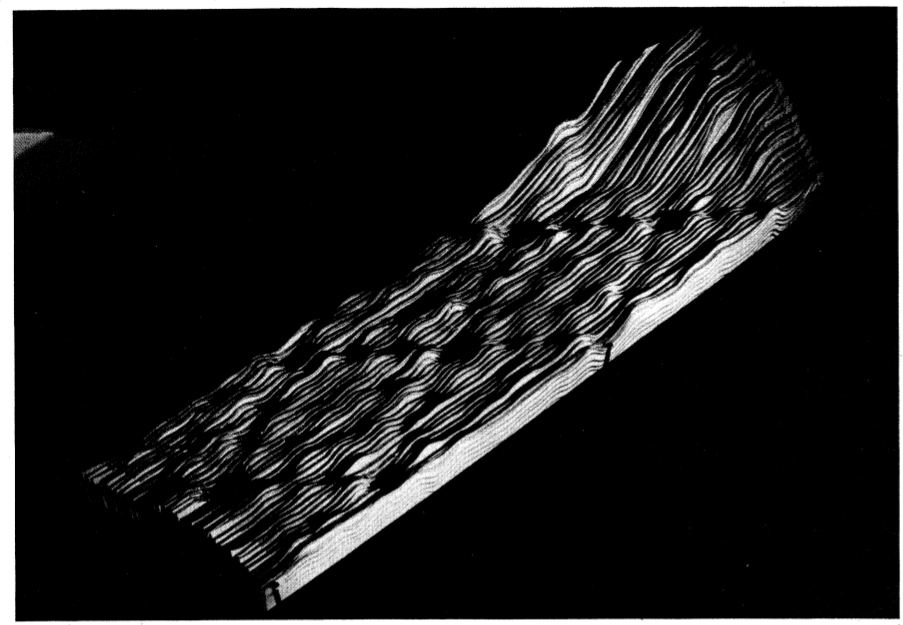
\includegraphics[width=10cm]{pics/silicium}
\caption{Erste Anwendung des Rastertunnelmikroskops 
\cite{binnig1983111}: 
Oberflächenrekonstruktion von Silizium(111) (siehe Millersche
Indizes im Theorieteil), welches eine komplexe (7x7) 
Überstrukturzelle besitzt}
 \label{fig:silicium}
\end{figure}

